%% Template para dissertação/tese na classe UFPEthesis
%% versão 0.9.2
%% (c) 2005 Paulo G. S. Fonseca
%% www.cin.ufpe.br/~paguso/ufpethesis

%% Carrega a classe ufpethesis
%% Opções: * Idiomas
%%           pt   - português (padrão)
%%           en   - inglês
%%         * Tipo do Texto
%%           bsc  - para monografias de graduação
%%           msc  - para dissertações de mestrado (padrão)
%%           qual - exame de qualificação doutorado
%%           prop - proposta de tese doutorado
%%           phd  - para teses de doutorado
%%         * Mídia
%%           scr  - para versão eletrônica (PDF) / consulte o guia do usuario
%%         * Estilo
%%           classic - estilo original à la TAOCP (deprecated)
%%           std     - novo estilo à la CUP (padrão)
%%         * Paginação
%%           oneside - para impressão em face única
%%           twoside - para impressão em frente e verso (padrão)
\documentclass[bsc, oneside]{UFPEThesis/ufpethesis}

%% Preâmbulo:
%% coloque aqui o seu preâmbulo LaTeX, i.e., declaração de pacotes,
%% (re)definições de macros, medidas, etc.

%% Identificação:

% Universidade
% e.g. \university{Universidade de Campinas}
% Na UFPE, comente a linha a seguir
\university{Universidade Federal de Pernambuco}

% Endereço (cidade)
% e.g. \address{Campinas}
% Na UFPE, comente a linha a seguir
% \address{<CIDADE DA IES>}

% Instituto ou Centro Acadêmico
% e.g. \institute{Centro de Ciências Exatas e da Natureza}
% Comente se não se aplicar
\institute{Centro de Informática}

% Departamento acadêmico
% e.g. \department{Departamento de Informática}
% Comente se não se aplicar
% \department{<NOME DO DEPARTAMENTO>}

% Programa de pós-graduação
% e.g. \program{Pós-graduação em Ciência da Computação}
\program{Bacharelado em Ciência da Computação}

% Área de titulação
% e.g. \majorfield{Ciência da Computação}
\majorfield{Ciência da Computação}

% Título da dissertação/tese
% e.g. \title{Sobre a conjectura $P=NP$}
\title{Previsão imediata de sequências de sinais de aúdio como método de redução de latência em transmissões online}

% Data da defesa
% e.g. \date{19 de fevereiro de 2003}
% \date{<DATA DA DEFESA>}

% Autor
% e.g. \author{José da Silva}
\author{Luiz Henrique Tavares Caúla}

% Orientador(a)
% Opção: [f] - para orientador do sexo feminino
% e.g. \adviser[f]{Profa. Dra. Maria Santos}
\adviser{Filipe Carlos de Albuquerque Calegario}

% Orientador(a)
% Opção: [f] - para orientador do sexo feminino
% e.g. \coadviser{Prof. Dr. Pedro Pedreira}
% Comente se não se aplicar
% \coadviser{NOME DO(DA) CO-ORIENTADOR(A)}

%% Inicio do documento
\begin{document}

%%
%% Parte pré-textual
%%
\frontmatter

% Folha de rosto
% Comente para ocultar
\frontpage

% Portada (apresentação)
% Comente para ocultar
\presentationpage

% Dedicatória
% Comente para ocultar
% \begin{dedicatory}
% <DIGITE A DEDICATÒRIA AQUI>
% \end{dedicatory}

% Agradecimentos
% Se preferir, crie um arquivo à parte e o inclua via \include{}
\acknowledgements
<DIGITE OS AGRADECIMENTOS AQUI>

% Epígrafe
% Comente para ocultar
% e.g.
%  \begin{epigraph}[Tarde, 1919]{Olavo Bilac}
%  Última flor do Lácio, inculta e bela,\\
%  És, a um tempo, esplendor e sepultura;\\
%  Ouro nativo, que, na ganga impura,\\
%  A bruta mina entre os cascalhos vela.
%  \end{epigraph}
% \begin{epigraph}[<NOTA>]{<AUTOR>}
% <DIGITE AQUI A CITAÇÂO>
% \end{epigraph}

% Resumo em Português
% Se preferir, crie um arquivo à parte e o inclua via \include{}
\resumo
\addcontentsline{toc}{chapter}{Resumo}

Devido ao curto tempo de reação a estímulos sonoros do aparelho auditivo humano, para performar em conjunto com outros artistas, músicos necessitam que haja pouca latência entre a saída de dos instrumentos de seus colegas e seu retorno. Dessa forma, proporcionar um ambiente colaborativo em tempo real via Internet torna-se um desafio pertinente na área de Computação Musical e Rede de Computadores. Algumas soluções procuram otimizar a conexão entre os computadores construindo infraestruturas dedicadas ou abandonam o requisito de tempo real ao entregar experiências assíncronas. No entanto, tais abordagens não abrangem, de forma síncrona, casos em que não haja acesso a uma conexão de alta velocidade ou que exista uma grande distância entre os participantes.

Este trabalho, portanto, investiga a possiblidade de predizer as próximas sequências imediatas de áudio, baseando-se em entradas passadas, considerando dois métodos - predição de sequências com LSTM (\textit{Long Short-Term Memory})\cite{lstm} e indexação de sequências usando DTW (\textit{Dynamic Time Warping})\cite{dtw}. De tal forma, espera-se que, não sendo necessária a espera pela saída do cliente transmissor, haja uma redução da percepção de latência por parte dos participantes.

\begin{keywords}
latência, áudio, predição de sequência, streaming, rollback, dtw, lstm
\end{keywords}


% Resumo em Inglês
% Se preferir, crie um arquivo à parte e o inclua via \include{}
% \abstract
% Palavras-chave do resumo em Inglês
% \begin{keywords}
% <DIGITE AS PALAVRAS-CHAVE AQUI>
% \end{keywords}

% Sumário
% Comente para ocultar
\tableofcontents

% Lista de figuras
% Comente para ocultar
\listoffigures

% Lista de tabelas
% Comente para ocultar
\listoftables



%%
%% Parte textual
%%
\mainmatter

% É aconselhável criar cada capítulo em um arquivo à parte, digamos
% "capitulo1.tex", "capitulo2.tex", ... "capituloN.tex" e depois
% incluí-los com:
\chapter{Introdução}

A performance artística musical, quando praticada em conjunto, requer alto nível de colaboração entre os participantes. Em música, sobretudo gêneros com tendências improvisacionais como \textit{jazz}, \textit{blues} e \textit{rock}, o ato de ouvir e reagir ao som de seus companheiros é tão importante quanto aquele produzido individualmente. Dessa forma, o \textit{feedback} auditivo de baixa latência dos instrumentos tocados é fundamental para que haja uma sensação fluida entre os participantes.

Normalmente, músicos performando em conjunto em um mesmo ambiente físico raramente experienciarão problemas relacionados à latência. No entanto, em um contexto de distanciamento social, encorajado durante à Pandemia de COVID-19, músicos ao redor do mundo viram-se obrigados a transferirem esse ambiente para um virtual \textit{online}. Além dos \textit{delays} causados pelas conversões de sinais analógicos para digitais e vice-versa e do tempo de escrita no \textit{buffer} em memória \cite{how_low_can_you_go}, a latência apresentada pela transmissão de pacotes pela Internet é o maior desafio para sobrepor, sendo o maior gargalo do processo de \textit{streaming} de áudio (\figref{fig:streaming_latencies}).

\begin{figure}[h]
\centering
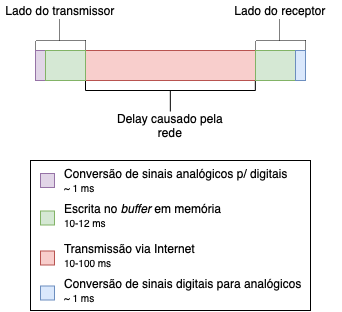
\includegraphics[width=0.5\textwidth]{images/streaming-latency.png}
\caption{Latências de cada fase do processo de \textit{streaming} de áudio pela Internet}
\label{fig:streaming_latencies}
\end{figure}

Aplicações comerciais de videoconferências, como o \textit{Zoom}, \textit{Google Meet} e \textit{FaceTime}  possuem sensibilidade de tempo para manter conversas compreensíveis - a \textit{Cisco} define a latência máxima aceitável de uma implementação \textit{VoIP} em até 150 ms \cite{cisco}. Este limite pode ser alcançado por conexões de velocidades medianas, mesmo considerando fatores como processamento de áudio e infraestruturas de rede compartilhadas. No entanto, para a prática colaborativa musical, onde tolerância máxima é bastante restrita - variando entre 10 ms e 55 ms \cite{mcphearson} - mostra-se inviável. Em ambientes de alta latência, músicos tendem a perceber incômodos e mudam a forma sobre como performam para adptarem-se. \cite{carot_low_latency}.

Para lidar com estes problemas, \textit{softwares} voltados especificamente para a colaboração musical \textit{online} apresentam uma variedade de abordagens diferentes. \textit{LoLa} \cite{lola}, \textit{SoundJack} \cite{soundjack} e \textit{JamKazam} \cite{jamkazam}, por exemplo, implementam otimizações na camada de rede - como conectar clientes diretamente entre si via \textit{P2P} (\textit{peer-to-peer}) - oferecendo latências razoáveis entre distâncias medianas. Outras aplicações, como o \textit{Jammr} \cite{jammr}, dispensam o requisito de tempo real e apresentam soluções assíncronas, onde os músicos ouvem os últimos quatro compassos tocados por seus companheiros em um \textit{loop} contínuo.

No entanto, tais abordagens não abrangem casos onde músicos residem entre grandes distâncias ou não é possível ter acesso a conexões dedicadas e \textit{hardwares} de alto valor financeiro, de forma a ainda manter uma performance síncrona.

Ao observar o contexto de videogames, encontramos requisitos de latência similares. Gêneros que utilizam reações como mecânica de jogabilidade, como luta e FPS (\textit{first-person shooter}), para oferecerem aos jogadores uma experiência fluida, necessitam de latências máximas de até 100 ms \cite{pubnub}. O algoritmo mais popular e efetivo para solucionar esse problema, \textit{Rollback Netcode} \cite{rollback}, baseia-se em prever os próximos \textit{inputs} imediatos dos jogadores e agindo antes mesmo que os dados de seu oponente sejam transmitidos; desta forma, removendo a necessidade inicial de espera. Uma vez que os \textit{inputs} são recebidos, estes são comparados com a previsão realizada e, caso sejam incongruentes entre si, o jogo é retornado ao estado anterior do momento da previsão inicial.

Por possuir contextos semelhantes, a mesma implementação baseada em previsões tem o potencial de resolver o problema descrito anteriormente para ambientes musicais colaborativos \textit{online}. Caso seja possível prever os próximos sinais digitais produzidos pelos artistas remotos, não haveria necessidade de espera e, portanto, a latência de rede tornaria-se irrelevante. É  evidente que, entretanto, por apresentar uma linearidade no tempo, não é possível retornar ao último momento da música anterior à previsão imediata. Portanto, é necessário que o modelo preditivo seja o mais acurado possível, visando minimizar a quantidade total de erros.

Dois ciclos de estudos foram explorados para explorar esse abordagem. Primeiramente, utilizando métodos de aprendizagem de máquina da biblioteca Keras \cite{keras}, especificamente LSTM, modelos foram gerados e treinados com cortes de 50 ms e 100 ms de arquivos de áudio no formato WAV. Uma vez treinado, a mesma sequência de treinamento foi usada, gerando uma nova sequência que a continuaria.

O segundo ciclo seguiu uma abordagem de criar um banco de dados de referência e, para cada nova entrada, identificava-se o corte com a duração desejava para previsão mais semelhante. O algoritmo de identificação usado foi o DTW, implementado pela biblioteca Librosa \cite{librosa}. Possuindo uma janela de referência, a próxima sequência do banco de dados era escolhida como predição da continuidade da música.


%%
%% Parte pós-textual
%%
\backmatter

% Apêndices
% Comente se não houver apêndices
\appendix

% É aconselhável criar cada apêndice em um arquivo à parte, digamos
% "apendice1.tex", "apendice.tex", ... "apendiceM.tex" e depois
% incluí-los com:
% \include{apendice1}
% \include{apendice2}
% ...
% \include{apendiceM}


% Bibliografia
% É aconselhável utilizar o BibTeX a partir de um arquivo, digamos "biblio.bib".
% Para ajuda na criação do arquivo .bib e utilização do BibTeX, recorra ao
% BibTeXpress em www.cin.ufpe.br/~paguso/bibtexpress
\nocite{*}
\bibliographystyle{ieeetr}
\bibliography{references}

% Cólofon
% Inclui uma pequena nota com referência à UFPEThesis
% Comente para omitir
% \colophon

%% Fim do documento
\end{document}
